\chapter{Test of the preamps frequency response}\label{app:preamp_frequency_response}
A test was made to get a view of the frequency response of the \gls{preamp}.

\section*{Materials and setup}
To measure the frequency response of the \gls{preamp}, the following materials are used:
\begin{itemize}
\item Digilent Analog Discovery 2 (Oscilloscope)
\item Digilent Waveforms 2015 (PC - software)
\end{itemize}


\begin{figure}[htbp!]
\centering
\begin{picture}(0,0)%
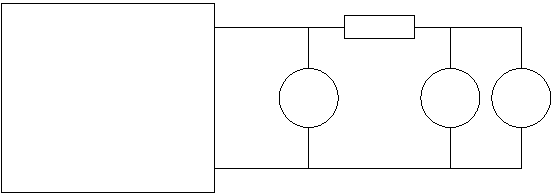
\includegraphics{guitar_output_phase_impedance.pdf}%
\end{picture}%
\setlength{\unitlength}{4144sp}%
%
\begingroup\makeatletter\ifx\SetFigFont\undefined%
\gdef\SetFigFont#1#2#3#4#5{%
  \reset@font\fontsize{#1}{#2pt}%
  \fontfamily{#3}\fontseries{#4}\fontshape{#5}%
  \selectfont}%
\fi\endgroup%
\begin{picture}(4205,1464)(4129,-2773)
\put(7426,-1996){Osc}%
\put(6346,-1996){Osc}%
\put(6346,-2176){Ch2}%
\put(7966,-1996){Osc}%
\put(8011,-2176){W1}%
\put(4681,-2086){DSP}%
\put(6346,-1771){+}%
\put(6346,-2401){-}%
\put(7426,-1771){+}%
\put(7471,-2401){-}%
\put(6796,-1591){Preamp}%
\put(7426,-2176){ch1}%
\end{picture}%
\caption{Setup for measuring phase of output impedance on a guitar.}
		\label{fig:appendix:preamp_frequency_response}
\end{figure}


\section*{Test procedure}
\begin{enumerate}
\item The materials are set up as in \autoref{fig:appendix:preamp_frequency_response}.
\item The Digilent Waveform 2015 is set as a Network analyser.
\item  The \gls{preamp} is set to have an gain of \SI{0}{\decibel}
\item  The network analyser is set to measure the input signal and the output signal from the \gls{preamp} from \SI{20}{\hertz} to \SI{20}{\kilo\hertz} with 10000 samples.
\item The measured data on the Osc ch1 and ch2 are used in the following formula: $\text{dB difference}= \text{ch2}-\text{ch1}$ which depends on the frequency. 
\item The data is plotted in MATLAB.
\end{enumerate}

\section*{Results}

\begin{figure}[htbp!]
	\centering
		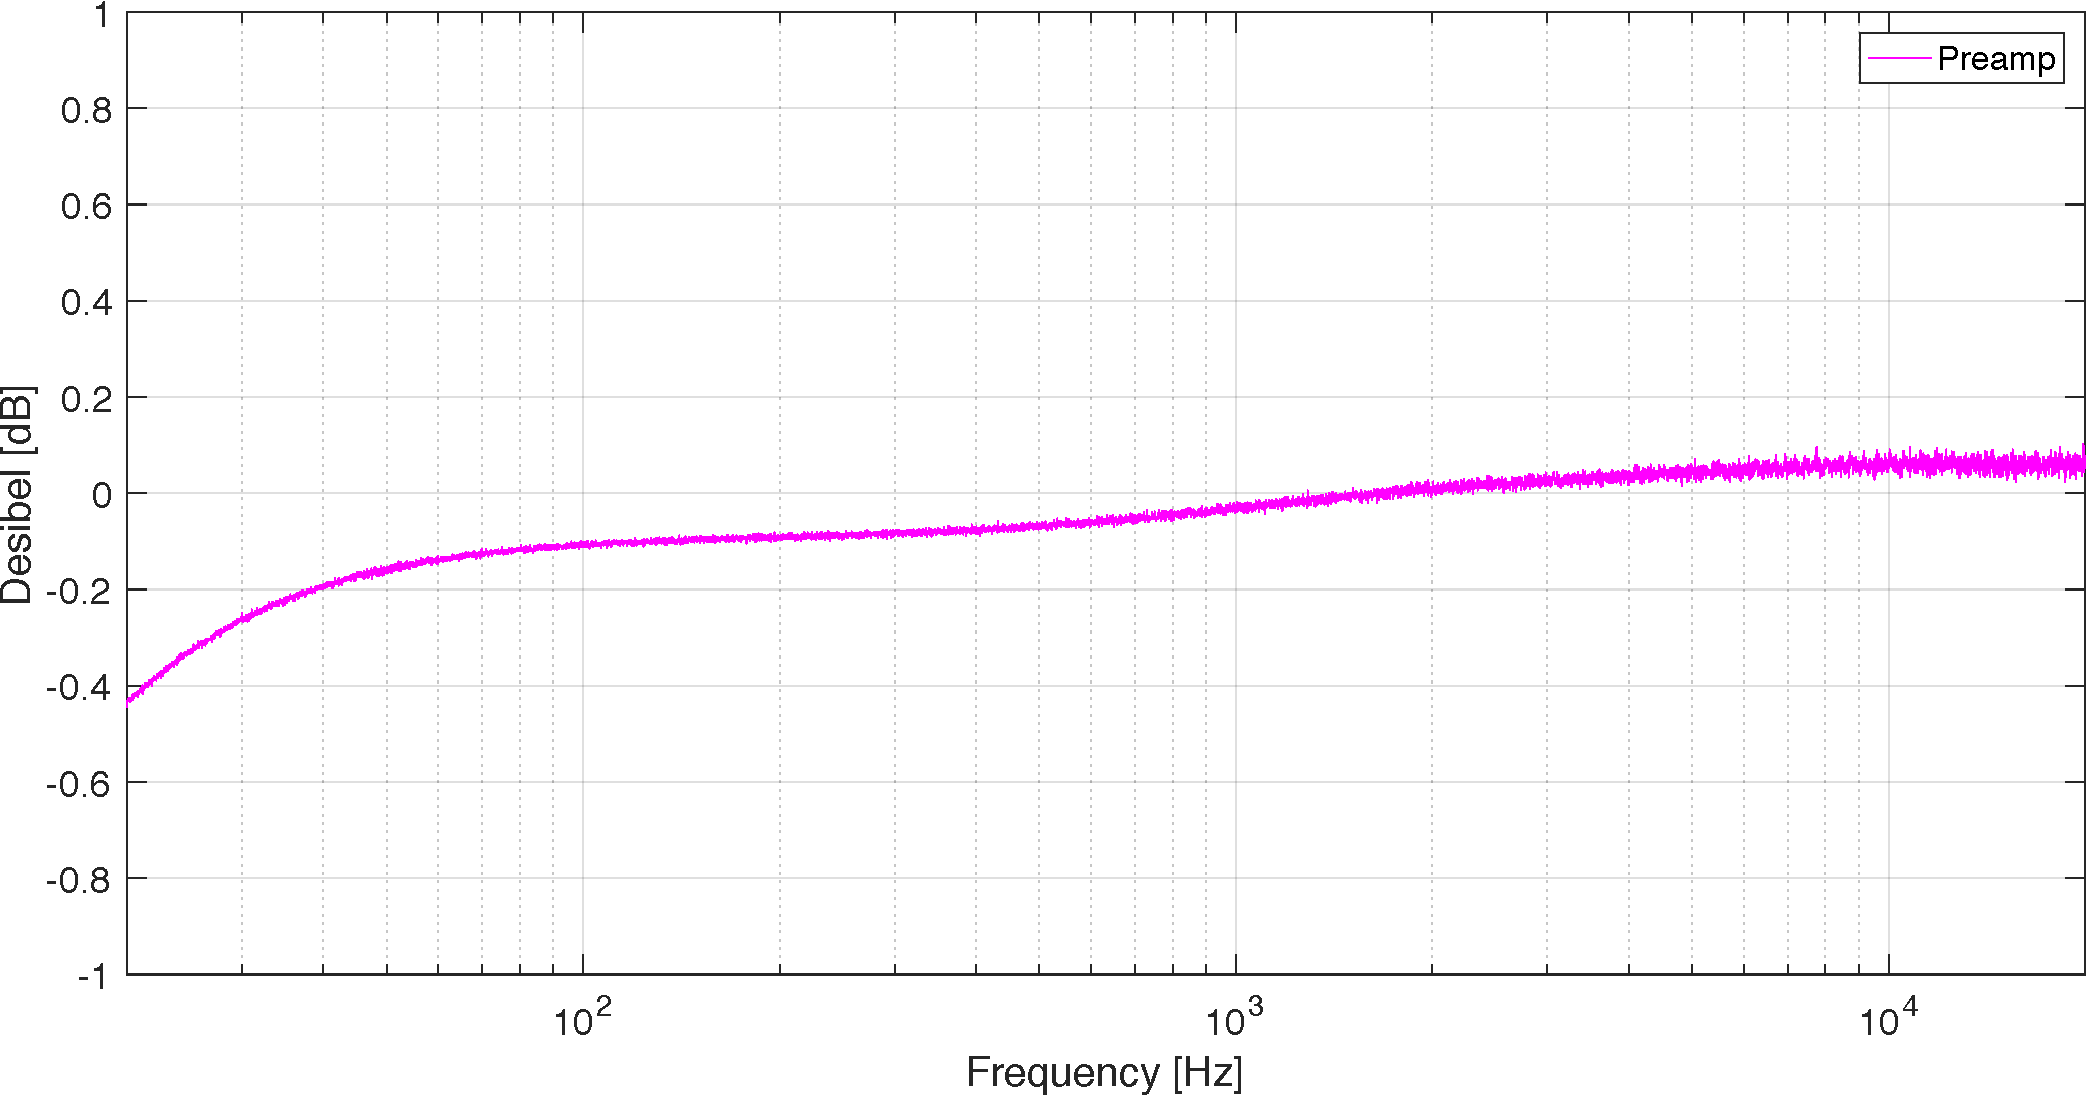
\includegraphics[width=1\textwidth]{preamp_frequency_responce.pdf}
		\caption{Measurement \gls{preamp}s magnitude response.}
		\label{fig:appendix:preamp_amplitude}
\end{figure}

\begin{figure}[htbp!]
	\centering
		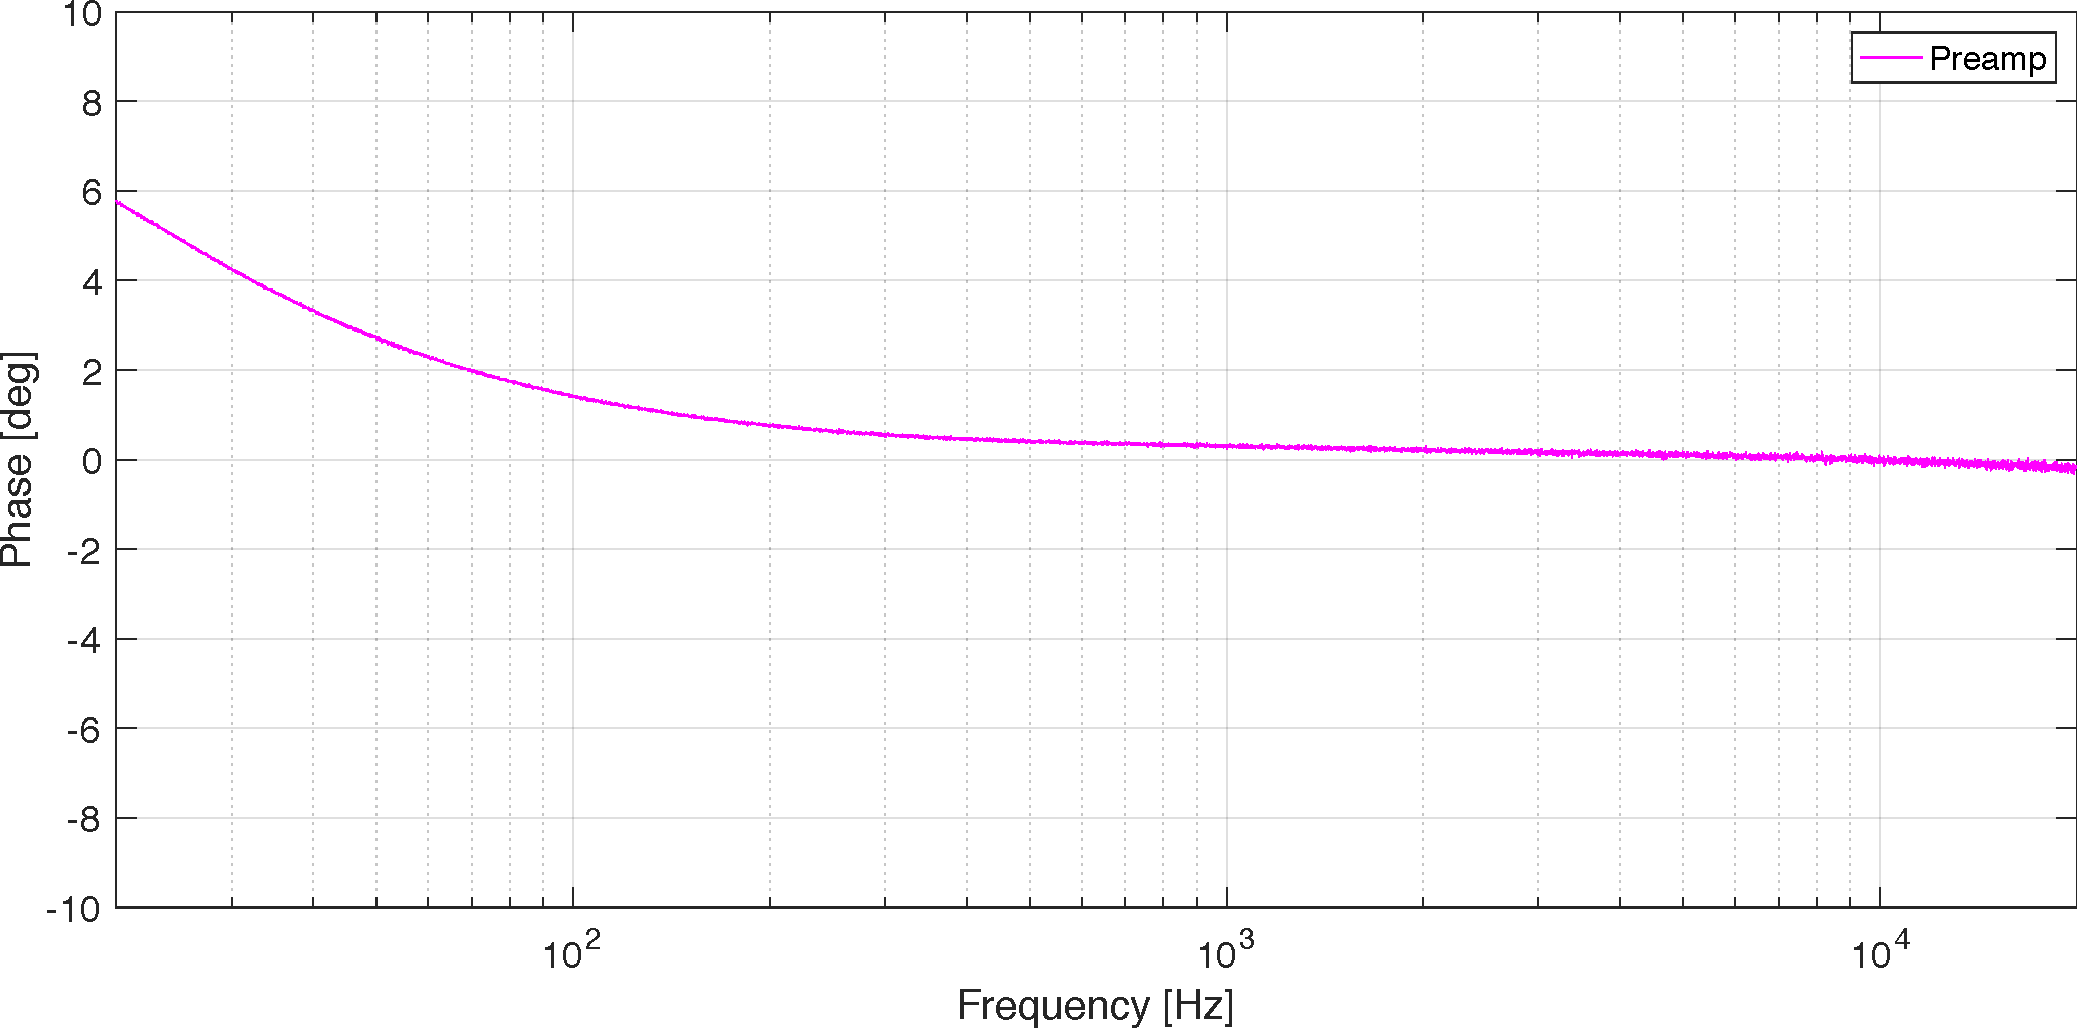
\includegraphics[width=1\textwidth]{preamp_frequency_responce_phase.pdf}
		\caption{Measurement of the \gls{preamp}s phase response.}
		\label{fig:appendix:preamp_phase}
\end{figure}
